% Options for packages loaded elsewhere
\PassOptionsToPackage{unicode}{hyperref}
\PassOptionsToPackage{hyphens}{url}
%
\documentclass[
  man,floatsintext]{apa6}
\usepackage{amsmath,amssymb}
\usepackage{iftex}
\ifPDFTeX
  \usepackage[T1]{fontenc}
  \usepackage[utf8]{inputenc}
  \usepackage{textcomp} % provide euro and other symbols
\else % if luatex or xetex
  \usepackage{unicode-math} % this also loads fontspec
  \defaultfontfeatures{Scale=MatchLowercase}
  \defaultfontfeatures[\rmfamily]{Ligatures=TeX,Scale=1}
\fi
\usepackage{lmodern}
\ifPDFTeX\else
  % xetex/luatex font selection
\fi
% Use upquote if available, for straight quotes in verbatim environments
\IfFileExists{upquote.sty}{\usepackage{upquote}}{}
\IfFileExists{microtype.sty}{% use microtype if available
  \usepackage[]{microtype}
  \UseMicrotypeSet[protrusion]{basicmath} % disable protrusion for tt fonts
}{}
\makeatletter
\@ifundefined{KOMAClassName}{% if non-KOMA class
  \IfFileExists{parskip.sty}{%
    \usepackage{parskip}
  }{% else
    \setlength{\parindent}{0pt}
    \setlength{\parskip}{6pt plus 2pt minus 1pt}}
}{% if KOMA class
  \KOMAoptions{parskip=half}}
\makeatother
\usepackage{xcolor}
\usepackage{graphicx}
\makeatletter
\def\maxwidth{\ifdim\Gin@nat@width>\linewidth\linewidth\else\Gin@nat@width\fi}
\def\maxheight{\ifdim\Gin@nat@height>\textheight\textheight\else\Gin@nat@height\fi}
\makeatother
% Scale images if necessary, so that they will not overflow the page
% margins by default, and it is still possible to overwrite the defaults
% using explicit options in \includegraphics[width, height, ...]{}
\setkeys{Gin}{width=\maxwidth,height=\maxheight,keepaspectratio}
% Set default figure placement to htbp
\makeatletter
\def\fps@figure{htbp}
\makeatother
\setlength{\emergencystretch}{3em} % prevent overfull lines
\providecommand{\tightlist}{%
  \setlength{\itemsep}{0pt}\setlength{\parskip}{0pt}}
\setcounter{secnumdepth}{-\maxdimen} % remove section numbering
% Make \paragraph and \subparagraph free-standing
\ifx\paragraph\undefined\else
  \let\oldparagraph\paragraph
  \renewcommand{\paragraph}[1]{\oldparagraph{#1}\mbox{}}
\fi
\ifx\subparagraph\undefined\else
  \let\oldsubparagraph\subparagraph
  \renewcommand{\subparagraph}[1]{\oldsubparagraph{#1}\mbox{}}
\fi
\ifLuaTeX
\usepackage[bidi=basic]{babel}
\else
\usepackage[bidi=default]{babel}
\fi
\babelprovide[main,import]{english}
% get rid of language-specific shorthands (see #6817):
\let\LanguageShortHands\languageshorthands
\def\languageshorthands#1{}
% Manuscript styling
\usepackage{upgreek}
\captionsetup{font=singlespacing,justification=justified}

% Table formatting
\usepackage{longtable}
\usepackage{lscape}
% \usepackage[counterclockwise]{rotating}   % Landscape page setup for large tables
\usepackage{multirow}		% Table styling
\usepackage{tabularx}		% Control Column width
\usepackage[flushleft]{threeparttable}	% Allows for three part tables with a specified notes section
\usepackage{threeparttablex}            % Lets threeparttable work with longtable

% Create new environments so endfloat can handle them
% \newenvironment{ltable}
%   {\begin{landscape}\centering\begin{threeparttable}}
%   {\end{threeparttable}\end{landscape}}
\newenvironment{lltable}{\begin{landscape}\centering\begin{ThreePartTable}}{\end{ThreePartTable}\end{landscape}}

% Enables adjusting longtable caption width to table width
% Solution found at http://golatex.de/longtable-mit-caption-so-breit-wie-die-tabelle-t15767.html
\makeatletter
\newcommand\LastLTentrywidth{1em}
\newlength\longtablewidth
\setlength{\longtablewidth}{1in}
\newcommand{\getlongtablewidth}{\begingroup \ifcsname LT@\roman{LT@tables}\endcsname \global\longtablewidth=0pt \renewcommand{\LT@entry}[2]{\global\advance\longtablewidth by ##2\relax\gdef\LastLTentrywidth{##2}}\@nameuse{LT@\roman{LT@tables}} \fi \endgroup}

% \setlength{\parindent}{0.5in}
% \setlength{\parskip}{0pt plus 0pt minus 0pt}

% Overwrite redefinition of paragraph and subparagraph by the default LaTeX template
% See https://github.com/crsh/papaja/issues/292
\makeatletter
\renewcommand{\paragraph}{\@startsection{paragraph}{4}{\parindent}%
  {0\baselineskip \@plus 0.2ex \@minus 0.2ex}%
  {-1em}%
  {\normalfont\normalsize\bfseries\itshape\typesectitle}}

\renewcommand{\subparagraph}[1]{\@startsection{subparagraph}{5}{1em}%
  {0\baselineskip \@plus 0.2ex \@minus 0.2ex}%
  {-\z@\relax}%
  {\normalfont\normalsize\itshape\hspace{\parindent}{#1}\textit{\addperi}}{\relax}}
\makeatother

% \usepackage{etoolbox}
\makeatletter
\patchcmd{\HyOrg@maketitle}
  {\section{\normalfont\normalsize\abstractname}}
  {\section*{\normalfont\normalsize\abstractname}}
  {}{\typeout{Failed to patch abstract.}}
\patchcmd{\HyOrg@maketitle}
  {\section{\protect\normalfont{\@title}}}
  {\section*{\protect\normalfont{\@title}}}
  {}{\typeout{Failed to patch title.}}
\makeatother

\usepackage{xpatch}
\makeatletter
\xapptocmd\appendix
  {\xapptocmd\section
    {\addcontentsline{toc}{section}{\appendixname\ifoneappendix\else~\theappendix\fi\\: #1}}
    {}{\InnerPatchFailed}%
  }
{}{\PatchFailed}
\keywords{effort discounting, registered report, specification curve analysis, need for cognition, $n$-back}
\usepackage{lineno}

\linenumbers
\usepackage{csquotes}
\usepackage{booktabs}
\usepackage{longtable}
\usepackage{array}
\usepackage{multirow}
\usepackage{wrapfig}
\usepackage{float}
\usepackage{colortbl}
\usepackage{pdflscape}
\usepackage{tabu}
\usepackage{threeparttable}
\usepackage{threeparttablex}
\usepackage[normalem]{ulem}
\usepackage{makecell}
\usepackage{xcolor}
\usepackage{setspace}\doublespacing
\usepackage[final]{pdfpages}
\usepackage{chngcntr}
\ifLuaTeX
  \usepackage{selnolig}  % disable illegal ligatures
\fi
\IfFileExists{bookmark.sty}{\usepackage{bookmark}}{\usepackage{hyperref}}
\IfFileExists{xurl.sty}{\usepackage{xurl}}{} % add URL line breaks if available
\urlstyle{same}
\hypersetup{
  pdftitle={Supplementary Material for the Registered Report titled: `Need for cognition is associated with a preference for higher task load in effort discounting'},
  pdfauthor={Josephine Zerna,1, Christoph Scheffel,1, Corinna Kührt1, \& Alexander Strobel1},
  pdflang={en-EN},
  pdfkeywords={effort discounting, registered report, specification curve analysis, need for cognition, \(n\)-back},
  hidelinks,
  pdfcreator={LaTeX via pandoc}}

\title{Supplementary Material for the Registered Report titled: `Need for cognition is associated with a preference for higher task load in effort discounting'}
\author{Josephine Zerna\textsuperscript{$\dagger{}$,1}, Christoph Scheffel\textsuperscript{$\dagger{}$,1}, Corinna Kührt\textsuperscript{1}, \& Alexander Strobel\textsuperscript{1}}
\date{}


\shorttitle{Supplement for CAD Paradigm}

\authornote{

The authors made the following contributions. Josephine Zerna: Conceptualization, Data curation, Methodology, Funding acquisition, Formal analysis, Investigation, Project administration, Software, Visualization, Writing - original draft, Writing - review \& editing; Christoph Scheffel: Conceptualization, Methodology, Funding acquisition, Investigation, Project administration, Software, Writing - review \& editing; Corinna Kührt: Formal analysis, Writing - review \& editing; Alexander Strobel: Conceptualization, Resources, Supervision, Funding acquistion, Writing - review \& editing. \textsuperscript{$\dagger{}$} Josephine Zerna and Christoph Scheffel contributed equally to this work.

Correspondence concerning this article should be addressed to Josephine Zerna, Zellescher Weg 17, 01069 Dresden, Germany. E-mail: \href{mailto:josephine.zerna@tu-dresden.de}{\nolinkurl{josephine.zerna@tu-dresden.de}}

}

\affiliation{\vspace{0.5cm}\textsuperscript{1} Faculty of Psychology, Technische Universität Dresden, 01069 Dresden, Germany}

\begin{document}
\maketitle

\newpage
\renewcommand\thesection{\Alph{section}}
\counterwithin{figure}{section}
\counterwithin{table}{section}
\setcounter{section}{19}
\setcounter{figure}{0}
\setcounter{table}{0}

\hypertarget{design-table}{%
\subsection{Design Table}\label{design-table}}

(Starts on next page)

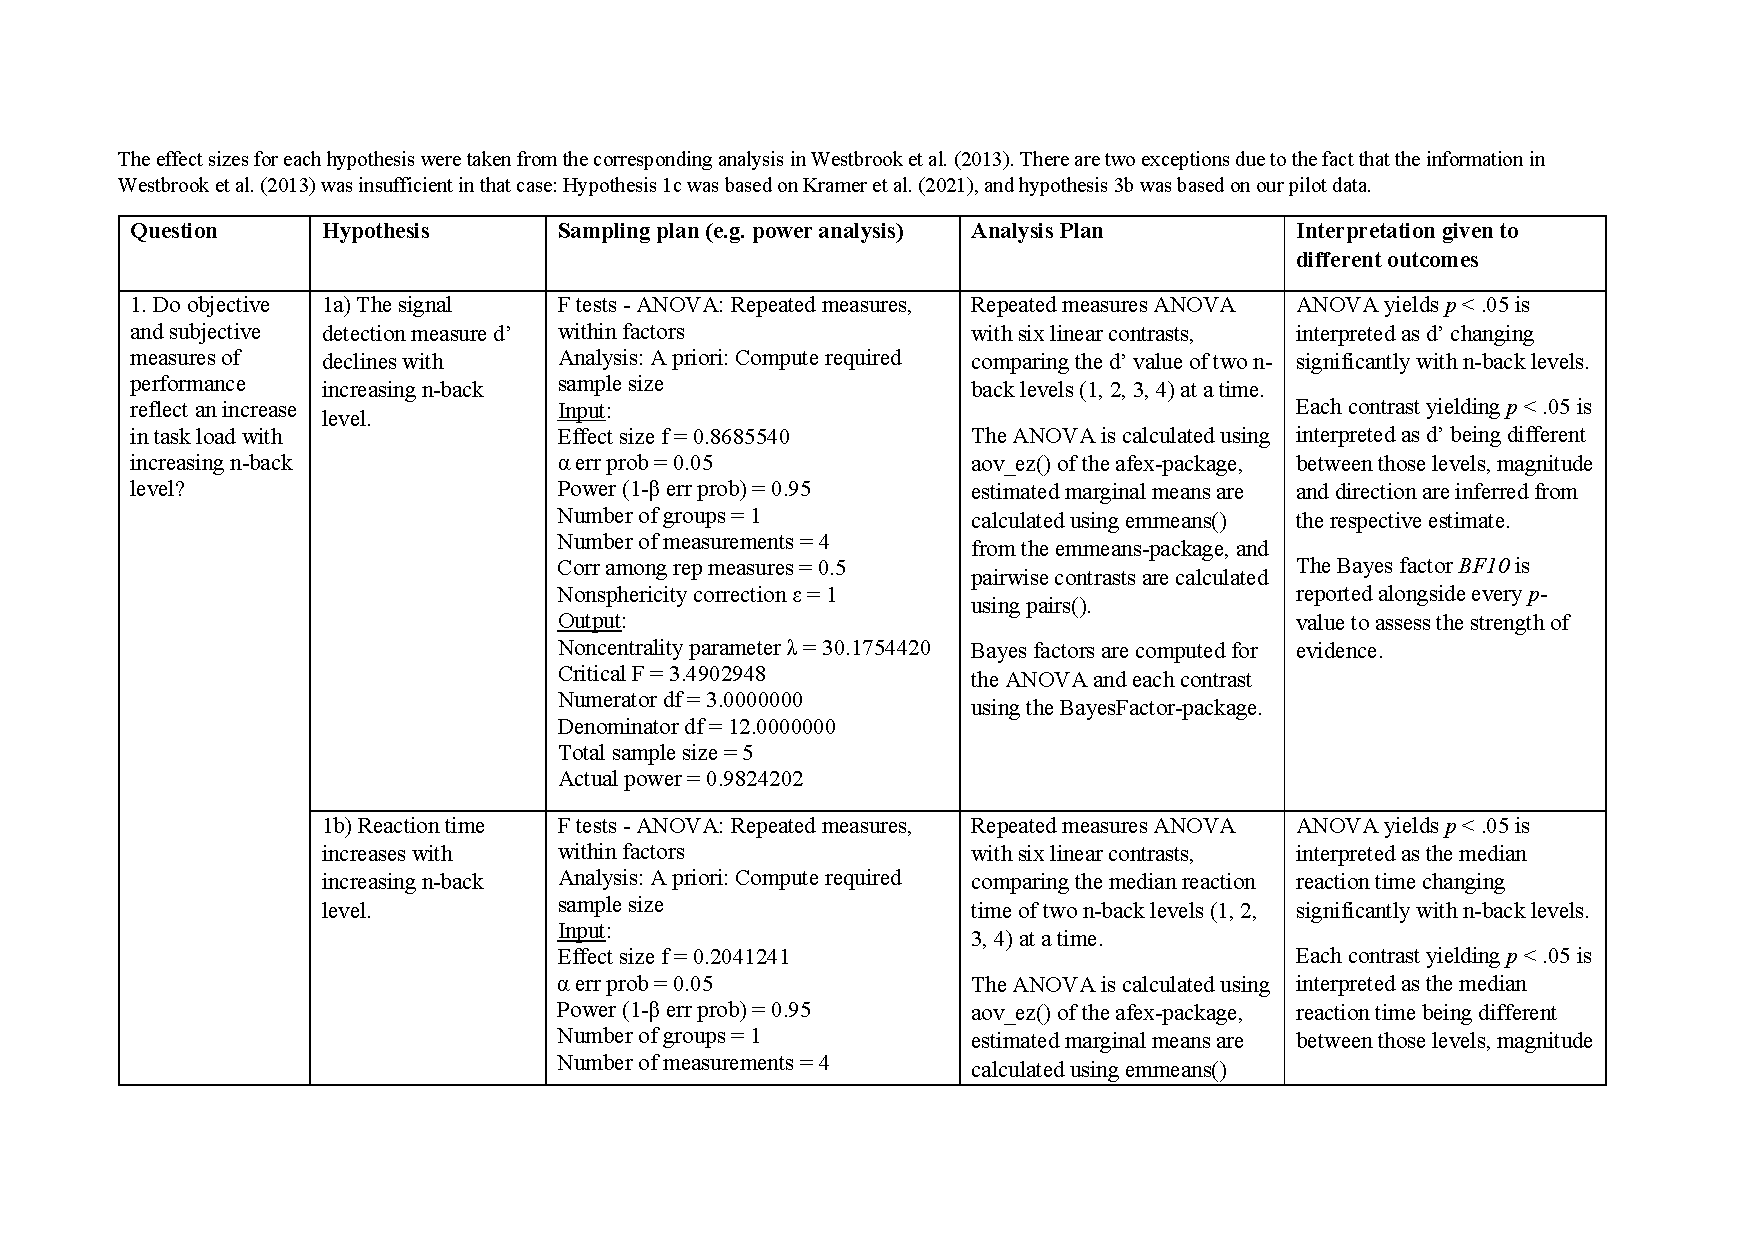
\includepdf[pages={-},landscape=true]{Design_Table_T1.pdf}

\newpage

\hypertarget{contrasts-tested-for-in-the-repeated-measures-anova}{%
\subsection{Contrasts tested for in the repeated measures ANOVA}\label{contrasts-tested-for-in-the-repeated-measures-anova}}

\begin{figure}[H]
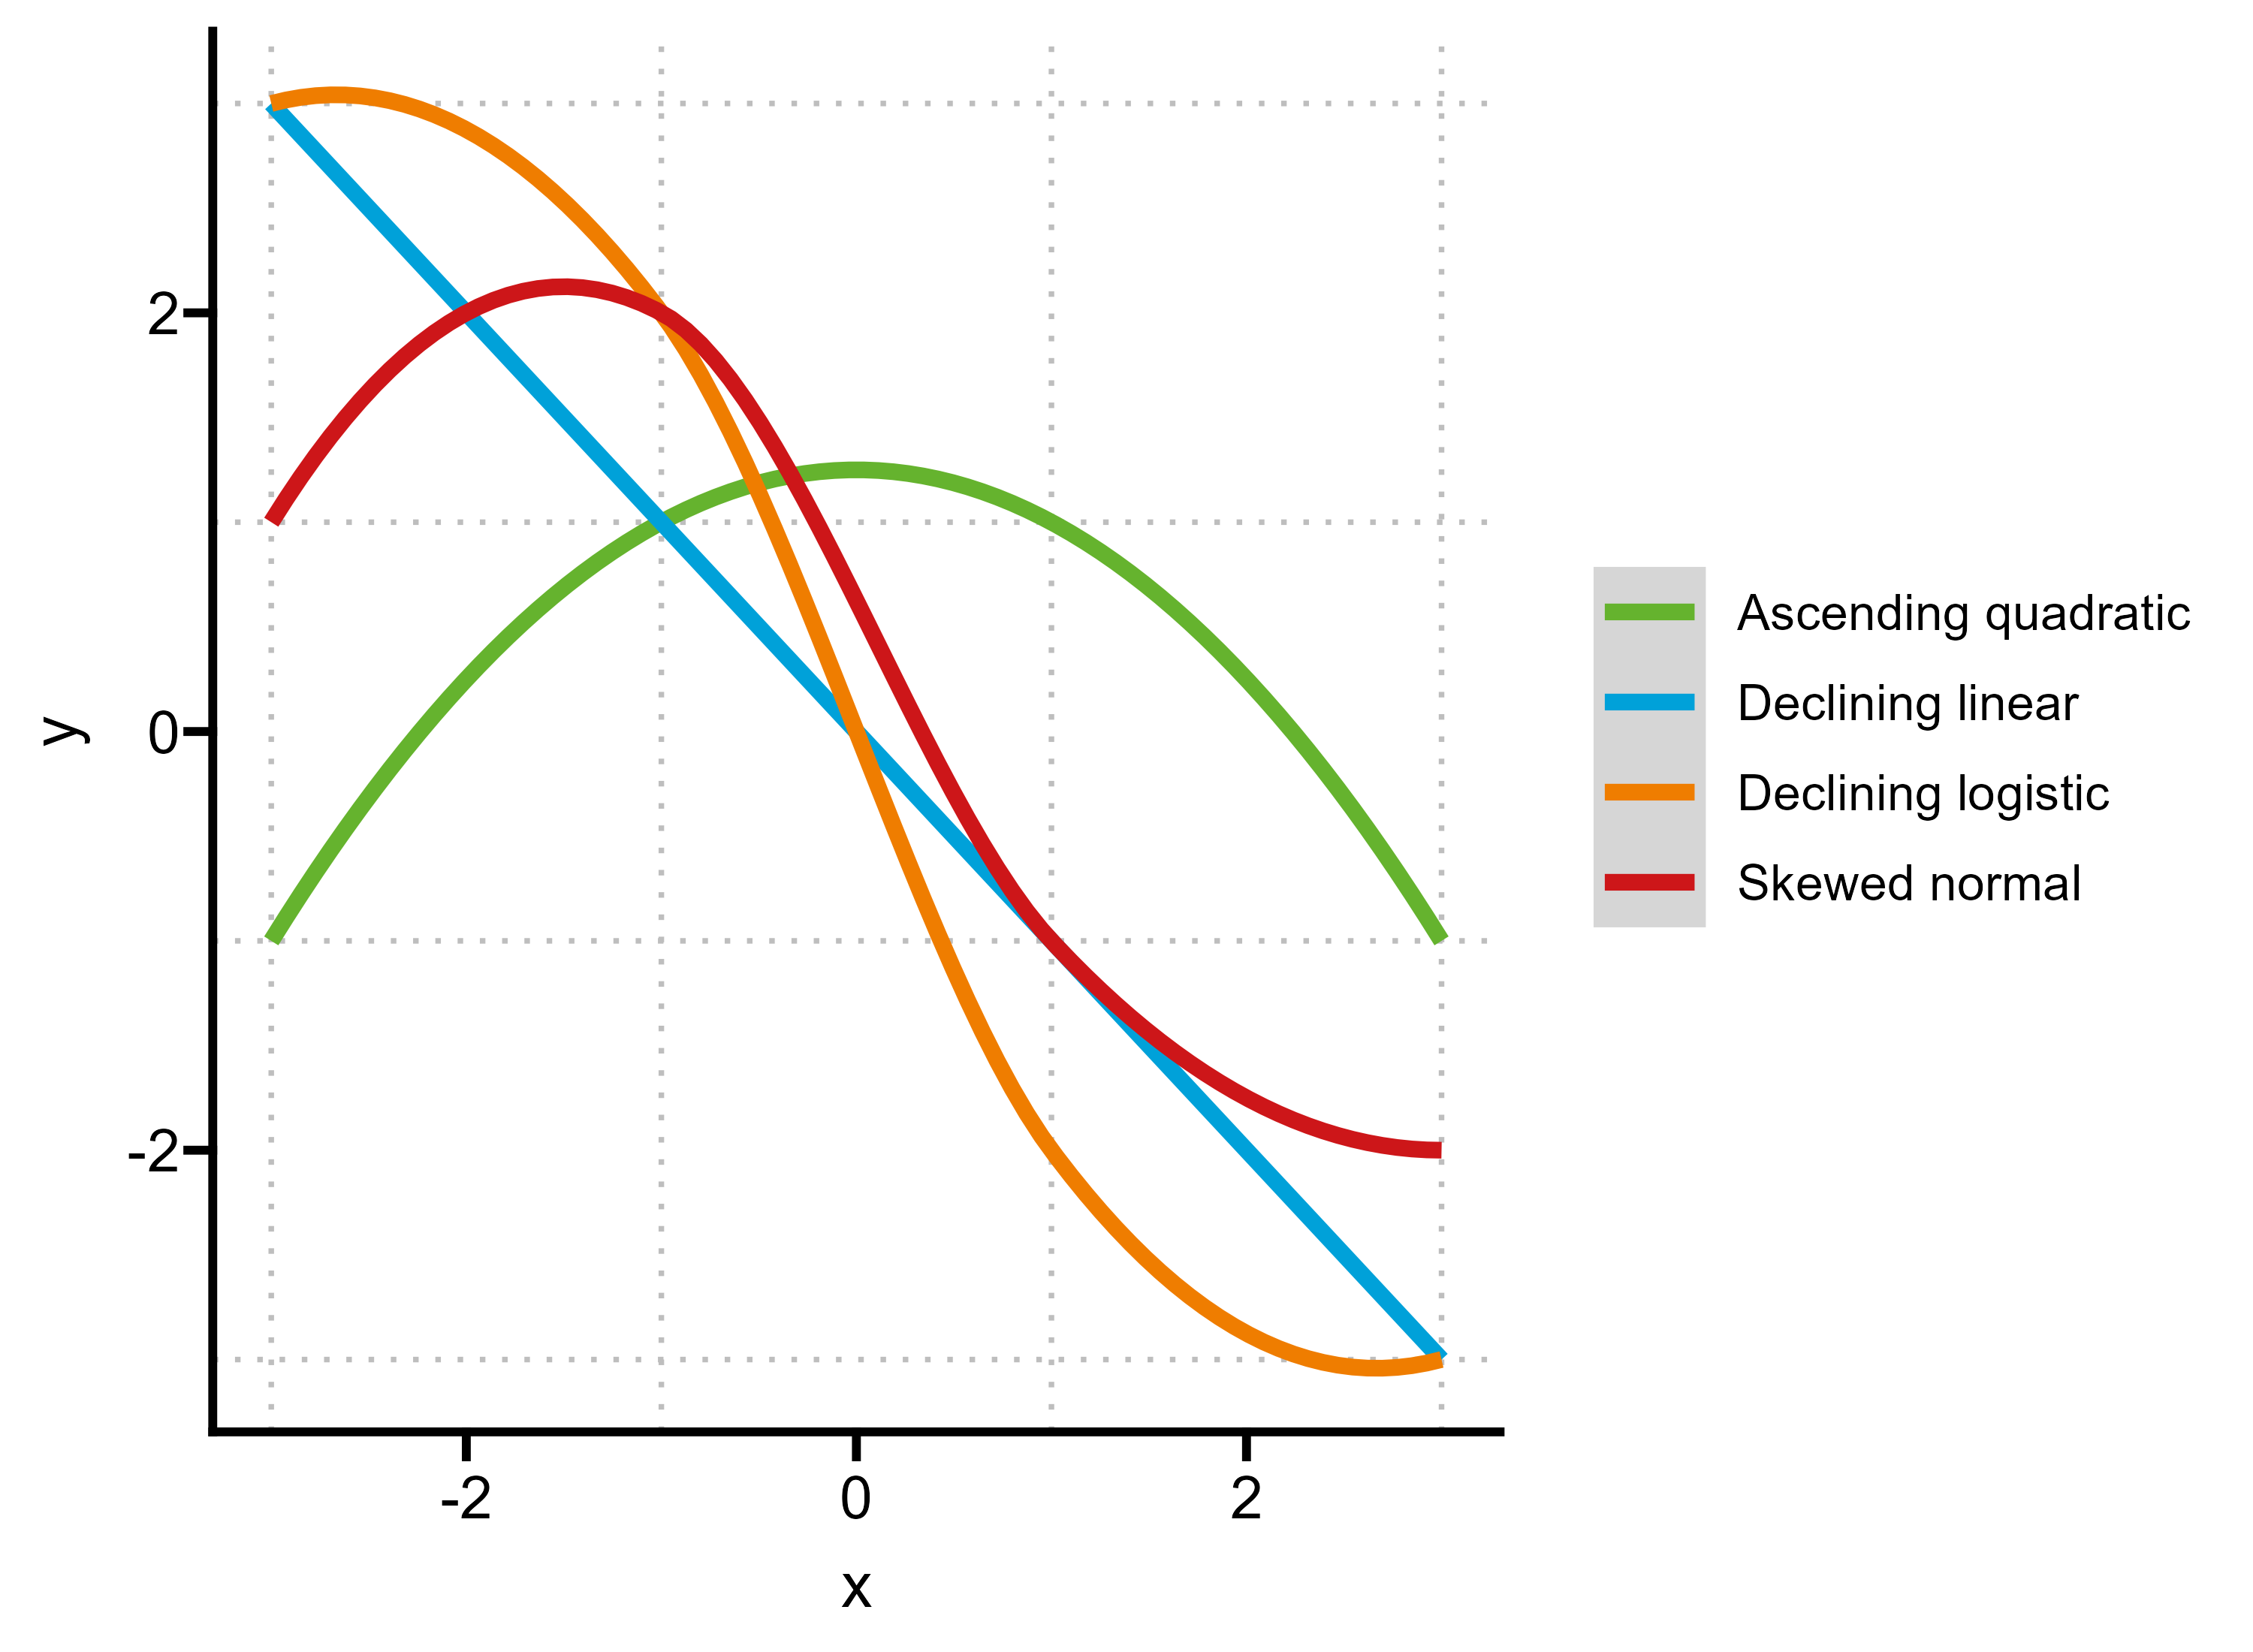
\includegraphics[width=\textwidth]{Figures/contrasts} \caption{Contrasts tested for in the repeated measures ANOVA that was used as a prerequisite for the multi level model of hypothesis 2b. Ascending quadratic (-1,1,1,-1), declining linear (3,1,-1,-3), declining logistic (3,2,-2,-3), and positively skewed normal (1,2,-1,-2). Figure available at osf.io/vnj8x/, under a CC-BY-4.0 license.}\label{fig:contrast-plot}
\end{figure}

\newpage

\hypertarget{hypothesis-1a-the-signal-detection-measure-d-declines-with-increasing-n-back-level.}{%
\subsection{\texorpdfstring{Hypothesis 1a: The signal detection measure \(d'\) declines with increasing \(n\)-back level.}{Hypothesis 1a: The signal detection measure d\textquotesingle{} declines with increasing n-back level.}}\label{hypothesis-1a-the-signal-detection-measure-d-declines-with-increasing-n-back-level.}}

ANOVA:

\(F(2.74, 315.51) = 197.18\), \(p < .001\), \(\hat{\eta}^2_G = .464\), 90\% CI \([.403, .516]\), \(\mathrm{BF}_{\textrm{10}} = 1.56 \times 10^{101}\)

Paired contrasts:

\begin{table}[H]

\begin{center}
\begin{threeparttable}

\caption{\label{tab:unnamed-chunk-1}Paired contrasts for the rmANOVA comparing $d'$ between $n$-back levels.}

\begin{tabular}{lllllllll}
\toprule
Contrast & \multicolumn{1}{c}{Estimate} & \multicolumn{1}{c}{$SE$} & \multicolumn{1}{c}{$df$} & \multicolumn{1}{c}{$t$} & \multicolumn{1}{c}{$p$} & \multicolumn{1}{c}{$\mathrm{BF}_{\textrm{10}}$} & \multicolumn{1}{c}{$\eta_{p}^{2}$} & \multicolumn{1}{c}{$95\% CI$}\\
\midrule
1 - 2 & 0.09 & 0.02 & 345.00 & 4.31 & 0.00 & 93,954.04 & 0.05 & {}[0.02, 1.00]\\
1 - 3 & 0.31 & 0.02 & 345.00 & 14.71 & 0.00 & $3.21 \times 10^{47}$ & 0.39 & {}[0.32, 1.00]\\
1 - 4 & 0.46 & 0.02 & 345.00 & 21.89 & 0.00 & $4.46 \times 10^{69}$ & 0.58 & {}[0.53, 1.00]\\
2 - 3 & 0.22 & 0.02 & 345.00 & 10.41 & 0.00 & $3.71 \times 10^{23}$ & 0.24 & {}[0.18, 1.00]\\
2 - 4 & 0.37 & 0.02 & 345.00 & 17.58 & 0.00 & $2.01 \times 10^{44}$ & 0.47 & {}[0.41, 1.00]\\
3 - 4 & 0.15 & 0.02 & 345.00 & 7.18 & 0.00 & $2.45 \times 10^{14}$ & 0.13 & {}[0.08, 1.00]\\
\bottomrule
\addlinespace
\end{tabular}

\begin{tablenotes}[para]
\normalsize{\textit{Note.} The column Contrast contains the $n$ of the $n$-back levels. $SE$ = standard error, $df$ = degrees of freedom, $t$ = $t$-statistic, $p$ = $p$-value, CI = confidence interval.}
\end{tablenotes}

\end{threeparttable}
\end{center}

\end{table}

\newpage

\hypertarget{hypothesis-1b-the-median-reaction-time-increases-with-increasing-n-back-level.}{%
\subsection{\texorpdfstring{Hypothesis 1b: The median reaction time increases with increasing \(n\)-back level.}{Hypothesis 1b: The median reaction time increases with increasing n-back level.}}\label{hypothesis-1b-the-median-reaction-time-increases-with-increasing-n-back-level.}}

ANOVA:

\(F(2.46, 283.05) = 98.67\), \(p < .001\), \(\hat{\eta}^2_G = .192\), 90\% CI \([.130, .248]\), \(\mathrm{BF}_{\textrm{10}} = 2.28 \times 10^{34}\)

Paired contrasts:

\begin{table}[H]

\begin{center}
\begin{threeparttable}

\caption{\label{tab:unnamed-chunk-2}Paired contrasts for the rmANOVA comparing the median reaction time between $n$-back levels.}

\begin{tabular}{lllllllll}
\toprule
Contrast & \multicolumn{1}{c}{Estimate} & \multicolumn{1}{c}{$SE$} & \multicolumn{1}{c}{$df$} & \multicolumn{1}{c}{$t$} & \multicolumn{1}{c}{$p$} & \multicolumn{1}{c}{$\mathrm{BF}_{\textrm{10}}$} & \multicolumn{1}{c}{$\eta_{p}^{2}$} & \multicolumn{1}{c}{$95\% CI$}\\
\midrule
1 - 2 & -0.11 & 0.01 & 345.00 & -11.76 & <.001 & $1.75 \times 10^{30}$ & 0.29 & {}[0.22, 1.00]\\
1 - 3 & -0.16 & 0.01 & 345.00 & -16.23 & <.001 & $8.80 \times 10^{45}$ & 0.43 & {}[0.37, 1.00]\\
1 - 4 & -0.12 & 0.01 & 345.00 & -12.47 & <.001 & $4.79 \times 10^{34}$ & 0.31 & {}[0.25, 1.00]\\
2 - 3 & -0.04 & 0.01 & 345.00 & -4.47 & <.001 & 5,538.45 & 0.05 & {}[0.02, 1.00]\\
2 - 4 & -0.01 & 0.01 & 345.00 & -0.71 & 0.894 & 0.10 & 1.45e-03 & {}[0.00, 1.00]\\
3 - 4 & 0.04 & 0.01 & 345.00 & 3.76 & 0.001 & $6.35 \times 10^{6}$ & 0.04 & {}[0.01, 1.00]\\
\bottomrule
\addlinespace
\end{tabular}

\begin{tablenotes}[para]
\normalsize{\textit{Note.} The column Contrast contains the $n$ of the $n$-back levels. $SE$ = standard error, $df$ = degrees of freedom, $t$ = $t$-statistic, $p$ = $p$-value, CI = confidence interval.}
\end{tablenotes}

\end{threeparttable}
\end{center}

\end{table}

\newpage

\hypertarget{hypothesis-1c-ratings-on-all-nasa-tlx-dimensions-increase-with-increasing-n-back-level.}{%
\subsection{\texorpdfstring{Hypothesis 1c: Ratings on all NASA-TLX dimensions increase with increasing \(n\)-back level.}{Hypothesis 1c: Ratings on all NASA-TLX dimensions increase with increasing n-back level.}}\label{hypothesis-1c-ratings-on-all-nasa-tlx-dimensions-increase-with-increasing-n-back-level.}}

Mental subscale ANOVA:

\(F(1.99, 228.35) = 274.47\), \(p < .001\), \(\hat{\eta}^2_G = .375\), 90\% CI \([.309, .432]\), \(\mathrm{BF}_{\textrm{10}} = 1.64 \times 10^{43}\)

Mental subscale paired contrasts:

\begin{table}[H]

\begin{center}
\begin{threeparttable}

\caption{\label{tab:unnamed-chunk-3}Paired contrasts for the rmANOVA comparing ratings on the NASA-TLX Mental subscale between $n$-back levels.}

\begin{tabular}{lllllllll}
\toprule
Contrast & \multicolumn{1}{c}{Estimate} & \multicolumn{1}{c}{$SE$} & \multicolumn{1}{c}{$df$} & \multicolumn{1}{c}{$t$} & \multicolumn{1}{c}{$p$} & \multicolumn{1}{c}{$\mathrm{BF}_{\textrm{10}}$} & \multicolumn{1}{c}{$\eta_{p}^{2}$} & \multicolumn{1}{c}{$95\% CI$}\\
\midrule
1 - 2 & -3.91 & 0.34 & 345.00 & -11.52 & <.001 & $1.32 \times 10^{23}$ & 0.28 & {}[0.21, 1.00]\\
1 - 3 & -7.43 & 0.34 & 345.00 & -21.91 & <.001 & $1.83 \times 10^{34}$ & 0.58 & {}[0.53, 1.00]\\
1 - 4 & -8.91 & 0.34 & 345.00 & -26.26 & <.001 & $9.87 \times 10^{36}$ & 0.67 & {}[0.62, 1.00]\\
2 - 3 & -3.53 & 0.34 & 345.00 & -10.40 & <.001 & $1.09 \times 10^{19}$ & 0.24 & {}[0.18, 1.00]\\
2 - 4 & -5.00 & 0.34 & 345.00 & -14.74 & <.001 & $3.64 \times 10^{22}$ & 0.39 & {}[0.32, 1.00]\\
3 - 4 & -1.47 & 0.34 & 345.00 & -4.35 & <.001 & $3.83 \times 10^{6}$ & 0.05 & {}[0.02, 1.00]\\
\bottomrule
\addlinespace
\end{tabular}

\begin{tablenotes}[para]
\normalsize{\textit{Note.} The column Contrast contains the $n$ of the $n$-back levels. $SE$ = standard error, $df$ = degrees of freedom, $t$ = $t$-statistic, $p$ = $p$-value, CI = confidence interval.}
\end{tablenotes}

\end{threeparttable}
\end{center}

\end{table}

\newpage

Physical subscale ANOVA:

\(F(1.68, 192.93) = 15.91\), \(p < .001\), \(\hat{\eta}^2_G = .041\), 90\% CI \([.009, .075]\), \(\mathrm{BF}_{\textrm{10}} = 60.54\)

Physical subscale paired contrasts:

\begin{table}[H]

\begin{center}
\begin{threeparttable}

\caption{\label{tab:unnamed-chunk-4}Paired contrasts for the rmANOVA comparing ratings on the NASA-TLX Physical subscale between $n$-back levels.}

\begin{tabular}{lllllllll}
\toprule
Contrast & \multicolumn{1}{c}{Estimate} & \multicolumn{1}{c}{$SE$} & \multicolumn{1}{c}{$df$} & \multicolumn{1}{c}{$t$} & \multicolumn{1}{c}{$p$} & \multicolumn{1}{c}{$\mathrm{BF}_{\textrm{10}}$} & \multicolumn{1}{c}{$\eta_{p}^{2}$} & \multicolumn{1}{c}{$95\% CI$}\\
\midrule
1 - 2 & -0.95 & 0.32 & 345.00 & -2.95 & 0.018 & 25.36 & 0.02 & {}[0.00, 1.00]\\
1 - 3 & -1.70 & 0.32 & 345.00 & -5.29 & <.001 & 602.59 & 0.08 & {}[0.04, 1.00]\\
1 - 4 & -2.04 & 0.32 & 345.00 & -6.37 & <.001 & 1,235.49 & 0.11 & {}[0.06, 1.00]\\
2 - 3 & -0.75 & 0.32 & 345.00 & -2.34 & 0.092 & 10.45 & 0.02 & {}[0.00, 1.00]\\
2 - 4 & -1.09 & 0.32 & 345.00 & -3.41 & 0.004 & 31.98 & 0.03 & {}[0.01, 1.00]\\
3 - 4 & -0.34 & 0.32 & 345.00 & -1.07 & 0.705 & 0.47 & 3.33e-03 & {}[0.00, 1.00]\\
\bottomrule
\addlinespace
\end{tabular}

\begin{tablenotes}[para]
\normalsize{\textit{Note.} The column Contrast contains the $n$ of the $n$-back levels. $SE$ = standard error, $df$ = degrees of freedom, $t$ = $t$-statistic, $p$ = $p$-value, CI = confidence interval.}
\end{tablenotes}

\end{threeparttable}
\end{center}

\end{table}

\newpage

Time subscale ANOVA:

\(F(2.21, 254.65) = 51.08\), \(p < .001\), \(\hat{\eta}^2_G = .117\), 90\% CI \([.065, .168]\), \(\mathrm{BF}_{\textrm{10}} = 3.94 \times 10^{9}\)

Time subscale paired contrasts:

\begin{table}[H]

\begin{center}
\begin{threeparttable}

\caption{\label{tab:unnamed-chunk-5}Paired contrasts for the rmANOVA comparing ratings on the NASA-TLX Time subscale between $n$-back levels.}

\begin{tabular}{lllllllll}
\toprule
Contrast & \multicolumn{1}{c}{Estimate} & \multicolumn{1}{c}{$SE$} & \multicolumn{1}{c}{$df$} & \multicolumn{1}{c}{$t$} & \multicolumn{1}{c}{$p$} & \multicolumn{1}{c}{$\mathrm{BF}_{\textrm{10}}$} & \multicolumn{1}{c}{$\eta_{p}^{2}$} & \multicolumn{1}{c}{$95\% CI$}\\
\midrule
1 - 2 & -1.95 & 0.43 & 345.00 & -4.53 & <.001 & 7,366.95 & 0.06 & {}[0.02, 1.00]\\
1 - 3 & -4.28 & 0.43 & 345.00 & -9.97 & <.001 & $3.09 \times 10^{10}$ & 0.22 & {}[0.16, 1.00]\\
1 - 4 & -4.65 & 0.43 & 345.00 & -10.81 & <.001 & $2.02 \times 10^{11}$ & 0.25 & {}[0.19, 1.00]\\
2 - 3 & -2.34 & 0.43 & 345.00 & -5.44 & <.001 & $9.62 \times 10^{6}$ & 0.08 & {}[0.04, 1.00]\\
2 - 4 & -2.70 & 0.43 & 345.00 & -6.28 & <.001 & $8.02 \times 10^{6}$ & 0.10 & {}[0.06, 1.00]\\
3 - 4 & -0.36 & 0.43 & 345.00 & -0.84 & 0.834 & 0.18 & 2.05e-03 & {}[0.00, 1.00]\\
\bottomrule
\addlinespace
\end{tabular}

\begin{tablenotes}[para]
\normalsize{\textit{Note.} The column Contrast contains the $n$ of the $n$-back levels. $SE$ = standard error, $df$ = degrees of freedom, $t$ = $t$-statistic, $p$ = $p$-value, CI = confidence interval.}
\end{tablenotes}

\end{threeparttable}
\end{center}

\end{table}

\newpage

Performance subscale ANOVA:

\(F(2.49, 285.97) = 95.33\), \(p < .001\), \(\hat{\eta}^2_G = .241\), 90\% CI \([.176, .299]\), \(\mathrm{BF}_{\textrm{10}} = 1.55 \times 10^{24}\)

Performance subscale paired contrasts:

\begin{table}[H]

\begin{center}
\begin{threeparttable}

\caption{\label{tab:unnamed-chunk-6}Paired contrasts for the rmANOVA comparing ratings on the NASA-TLX Performance subscale between $n$-back levels.}

\begin{tabular}{lllllllll}
\toprule
Contrast & \multicolumn{1}{c}{Estimate} & \multicolumn{1}{c}{$SE$} & \multicolumn{1}{c}{$df$} & \multicolumn{1}{c}{$t$} & \multicolumn{1}{c}{$p$} & \multicolumn{1}{c}{$\mathrm{BF}_{\textrm{10}}$} & \multicolumn{1}{c}{$\eta_{p}^{2}$} & \multicolumn{1}{c}{$95\% CI$}\\
\midrule
1 - 2 & 2.07 & 0.40 & 345.00 & 5.13 & <.001 & 80,590.41 & 0.07 & {}[0.03, 1.00]\\
1 - 3 & 5.14 & 0.40 & 345.00 & 12.74 & <.001 & $1.23 \times 10^{19}$ & 0.32 & {}[0.26, 1.00]\\
1 - 4 & 6.03 & 0.40 & 345.00 & 14.96 & <.001 & $2.36 \times 10^{19}$ & 0.39 & {}[0.33, 1.00]\\
2 - 3 & 3.07 & 0.40 & 345.00 & 7.61 & <.001 & $8.72 \times 10^{12}$ & 0.14 & {}[0.09, 1.00]\\
2 - 4 & 3.97 & 0.40 & 345.00 & 9.83 & <.001 & $4.20 \times 10^{12}$ & 0.22 & {}[0.16, 1.00]\\
3 - 4 & 0.90 & 0.40 & 345.00 & 2.22 & 0.119 & 2.35 & 0.01 & {}[0.00, 1.00]\\
\bottomrule
\addlinespace
\end{tabular}

\begin{tablenotes}[para]
\normalsize{\textit{Note.} The column Contrast contains the $n$ of the $n$-back levels. $SE$ = standard error, $df$ = degrees of freedom, $t$ = $t$-statistic, $p$ = $p$-value, CI = confidence interval.}
\end{tablenotes}

\end{threeparttable}
\end{center}

\end{table}

\newpage

Effort subscale ANOVA:

\(F(2.20, 253.06) = 203.82\), \(p < .001\), \(\hat{\eta}^2_G = .316\), 90\% CI \([.250, .375]\), \(\mathrm{BF}_{\textrm{10}} = 2.47 \times 10^{34}\)

Effort subscale paired contrasts:

\begin{table}[H]

\begin{center}
\begin{threeparttable}

\caption{\label{tab:unnamed-chunk-7}Paired contrasts for the rmANOVA comparing ratings on the NASA-TLX Effort subscale between $n$-back levels.}

\begin{tabular}{lllllllll}
\toprule
Contrast & \multicolumn{1}{c}{Estimate} & \multicolumn{1}{c}{$SE$} & \multicolumn{1}{c}{$df$} & \multicolumn{1}{c}{$t$} & \multicolumn{1}{c}{$p$} & \multicolumn{1}{c}{$\mathrm{BF}_{\textrm{10}}$} & \multicolumn{1}{c}{$\eta_{p}^{2}$} & \multicolumn{1}{c}{$95\% CI$}\\
\midrule
1 - 2 & -4.23 & 0.34 & 345.00 & -12.35 & <.001 & $4.24 \times 10^{19}$ & 0.31 & {}[0.24, 1.00]\\
1 - 3 & -6.80 & 0.34 & 345.00 & -19.84 & <.001 & $4.25 \times 10^{29}$ & 0.53 & {}[0.48, 1.00]\\
1 - 4 & -7.73 & 0.34 & 345.00 & -22.56 & <.001 & $1.47 \times 10^{32}$ & 0.60 & {}[0.55, 1.00]\\
2 - 3 & -2.57 & 0.34 & 345.00 & -7.49 & <.001 & $3.85 \times 10^{12}$ & 0.14 & {}[0.09, 1.00]\\
2 - 4 & -3.50 & 0.34 & 345.00 & -10.21 & <.001 & $3.33 \times 10^{15}$ & 0.23 & {}[0.17, 1.00]\\
3 - 4 & -0.93 & 0.34 & 345.00 & -2.72 & 0.035 & 174.38 & 0.02 & {}[0.00, 1.00]\\
\bottomrule
\addlinespace
\end{tabular}

\begin{tablenotes}[para]
\normalsize{\textit{Note.} The column Contrast contains the $n$ of the $n$-back levels. $SE$ = standard error, $df$ = degrees of freedom, $t$ = $t$-statistic, $p$ = $p$-value, CI = confidence interval.}
\end{tablenotes}

\end{threeparttable}
\end{center}

\end{table}

\newpage

Frustration subscale ANOVA:

\(F(2.50, 287.66) = 68.06\), \(p < .001\), \(\hat{\eta}^2_G = .172\), 90\% CI \([.112, .227]\), \(\mathrm{BF}_{\textrm{10}} = 5.26 \times 10^{15}\)

Frustration subscale paired contrasts:

\begin{table}[H]

\begin{center}
\begin{threeparttable}

\caption{\label{tab:unnamed-chunk-8}Paired contrasts for the rmANOVA comparing ratings on the NASA-TLX Frustration subscale between $n$-back levels.}

\begin{tabular}{lllllllll}
\toprule
Contrast & \multicolumn{1}{c}{Estimate} & \multicolumn{1}{c}{$SE$} & \multicolumn{1}{c}{$df$} & \multicolumn{1}{c}{$t$} & \multicolumn{1}{c}{$p$} & \multicolumn{1}{c}{$\mathrm{BF}_{\textrm{10}}$} & \multicolumn{1}{c}{$\eta_{p}^{2}$} & \multicolumn{1}{c}{$95\% CI$}\\
\midrule
1 - 2 & -2.17 & 0.43 & 345.00 & -4.99 & <.001 & 67,280.87 & 0.07 & {}[0.03, 1.00]\\
1 - 3 & -4.76 & 0.43 & 345.00 & -10.94 & <.001 & $8.22 \times 10^{14}$ & 0.26 & {}[0.20, 1.00]\\
1 - 4 & -5.57 & 0.43 & 345.00 & -12.80 & <.001 & $2.34 \times 10^{15}$ & 0.32 & {}[0.26, 1.00]\\
2 - 3 & -2.59 & 0.43 & 345.00 & -5.95 & <.001 & $6.41 \times 10^{7}$ & 0.09 & {}[0.05, 1.00]\\
2 - 4 & -3.40 & 0.43 & 345.00 & -7.81 & <.001 & $6.16 \times 10^{8}$ & 0.15 & {}[0.10, 1.00]\\
3 - 4 & -0.81 & 0.43 & 345.00 & -1.86 & 0.246 & 0.92 & 9.96e-03 & {}[0.00, 1.00]\\
\bottomrule
\addlinespace
\end{tabular}

\begin{tablenotes}[para]
\normalsize{\textit{Note.} The column Contrast contains the $n$ of the $n$-back levels. $SE$ = standard error, $df$ = degrees of freedom, $t$ = $t$-statistic, $p$ = $p$-value, CI = confidence interval.}
\end{tablenotes}

\end{threeparttable}
\end{center}

\end{table}

\newpage

\hypertarget{hypothesis-2a-subjective-values-decline-with-increasing-n-back-level.}{%
\subsection{\texorpdfstring{Hypothesis 2a: Subjective values decline with increasing \(n\)-back level.}{Hypothesis 2a: Subjective values decline with increasing n-back level.}}\label{hypothesis-2a-subjective-values-decline-with-increasing-n-back-level.}}

ANOVA:

\(F(1.98, 227.98) = 65.65\), \(p < .001\), \(\hat{\eta}^2_G = .288\), 90\% CI \([.222, .347]\), \(\mathrm{BF}_{\textrm{10}} = 1.58 \times 10^{64}\)

Pre-defined contrasts:

\begin{table}[H]

\begin{center}
\begin{threeparttable}

\caption{\label{tab:unnamed-chunk-9}Contrasts for the rmANOVA comparing the subjective values between $n$-back levels.}

\begin{tabular}{llllllll}
\toprule
Contrast & \multicolumn{1}{c}{Estimate} & \multicolumn{1}{c}{$SE$} & \multicolumn{1}{c}{$df$} & \multicolumn{1}{c}{$t$} & \multicolumn{1}{c}{$p$} & \multicolumn{1}{c}{$\eta_{p}^{2}$} & \multicolumn{1}{c}{$95\% CI$}\\
\midrule
Declining Linear & 1.11 & 0.08 & 345.00 & 13.41 & <.001 & 0.34 & {}[0.28, 1.00]\\
Ascending Quadratic & 0.15 & 0.04 & 345.00 & 4.14 & <.001 & 0.05 & {}[0.02, 1.00]\\
Declining Logistic & 1.22 & 0.09 & 345.00 & 12.97 & <.001 & 0.33 & {}[0.26, 1.00]\\
Positively Skewed Normal & 0.75 & 0.06 & 345.00 & 12.74 & <.001 & 0.32 & {}[0.26, 1.00]\\
\bottomrule
\addlinespace
\end{tabular}

\begin{tablenotes}[para]
\normalsize{\textit{Note.} $SE$ = standard error, $df$ = degrees of freedom, $t$ = $t$-statistic, $p$ = $p$-value, CI = confidence interval.}
\end{tablenotes}

\end{threeparttable}
\end{center}

\end{table}

\newpage

\hypertarget{hypothesis-2b-subjective-values-decline-with-increasing-n-back-level-even-after-controlling-for-declining-task-performance-measured-by-signal-detection-d-and-reaction-time.}{%
\subsection{\texorpdfstring{Hypothesis 2b: Subjective values decline with increasing \(n\)-back level, even after controlling for declining task performance measured by signal detection d' and reaction time.}{Hypothesis 2b: Subjective values decline with increasing n-back level, even after controlling for declining task performance measured by signal detection d' and reaction time.}}\label{hypothesis-2b-subjective-values-decline-with-increasing-n-back-level-even-after-controlling-for-declining-task-performance-measured-by-signal-detection-d-and-reaction-time.}}

Multi level model:

\begin{table}[H]

\begin{center}
\begin{threeparttable}

\caption{\label{tab:unnamed-chunk-10}Results of the multi level model on the influence of n-back level (as a declining logistic contrast) and task performance on subjective values.}

\begin{tabular}{llllllll}
\toprule
Parameter & \multicolumn{1}{c}{Beta} & \multicolumn{1}{c}{$SE$} & \multicolumn{1}{c}{$df$} & \multicolumn{1}{c}{$t$-value} & \multicolumn{1}{c}{$p$-value} & \multicolumn{1}{c}{$f^{2}$} & \multicolumn{1}{c}{Random Effects (SD)}\\
\midrule
Intercept & 0.81 & 0.01 & 115.00 & 78.68 & <.001 &  & 0.09\\
n-back level & 0.03 & 0.00 & 797.54 & 9.99 & <.001 & 0.21 & \\
d' & 0.21 & 0.03 & 797.63 & 6.28 & <.001 & 0.05 & \\
median RT & 0.03 & 0.07 & 797.80 & 0.42 & 0.674 & 0.00 & \\
\bottomrule
\addlinespace
\end{tabular}

\begin{tablenotes}[para]
\normalsize{\textit{Note.} $SE$ = standard error, $df$ = degrees of freedom, $SD$ = standard deviation.}
\end{tablenotes}

\end{threeparttable}
\end{center}

\end{table}

The final model had an effect size of \(f^{2}=\) 0.21 for the \(n\)-back levels and \(f^{2}=\) 0.05 for \(d'\).
This means that the \(n\)-back level explained 20.67\% and \(d'\) explained 4.90\% of variance in SVs relative to the unexplained variance, respectively.
The beta coefficient indicated that with every 1-unit increase in \(d'\), the SV increased by 0.21.
The effect size of the median RT was \(f^{2}=\) 0.00.
The Bayes Factor of the full model against the null model was \(\mathrm{BF}_{\textrm{10}} = 7.83 \times 10^{29} \pm 16.28\%\).

\newpage

\hypertarget{hypothesis-3a-participants-with-higher-nfc-scores-have-higher-subjective-values-for-2--and-3-back-but-lower-subjective-values-for-1-back-than-participants-with-lower-nfc-scores.}{%
\subsection{Hypothesis 3a: Participants with higher NFC scores have higher subjective values for 2- and 3-back but lower subjective values for 1-back than participants with lower NFC scores.}\label{hypothesis-3a-participants-with-higher-nfc-scores-have-higher-subjective-values-for-2--and-3-back-but-lower-subjective-values-for-1-back-than-participants-with-lower-nfc-scores.}}

ANOVA:

Main effect level: \(F(1, 114) = 9.13\), \(p = .003\), \(\hat{\eta}^2_G = .040\), 90\% CI \([.002, .115]\), \(\mathrm{BF}_{\textrm{10}} = 12.68 \pm 0.00\%\)

Main effect NFC group: \(F(1, 114) = 3.18\), \(p = .077\), \(\hat{\eta}^2_G = .013\), 90\% CI \([.000, .068]\), \(\mathrm{BF}_{\textrm{10}} = 0.56 \pm 0.03\%\)

Interaction: \(F(1, 114) = 0.46\), \(p = .499\), \(\hat{\eta}^2_G = .002\), 90\% CI \([.000, .037]\)

Contrast for main effect level:

\begin{table}[H]

\begin{center}
\begin{threeparttable}

\caption{\label{tab:unnamed-chunk-11}Paired contrast for the rmANOVA comparing the influence of Need for Cognition group and $n$-back level on difference scores of subjective values.}

\begin{tabular}{lllllllll}
\toprule
Contrast & \multicolumn{1}{c}{Estimate} & \multicolumn{1}{c}{$SE$} & \multicolumn{1}{c}{$df$} & \multicolumn{1}{c}{$t$} & \multicolumn{1}{c}{$p$} & \multicolumn{1}{c}{$\mathrm{BF}_{\textrm{10}}$} & \multicolumn{1}{c}{$\eta_{p}^{2}$} & \multicolumn{1}{c}{$95\% CI$}\\
\midrule
1-2 - 2-3 & -0.08 & 0.03 & 114.00 & -3.02 & 0.003 & 12.68 & 0.07 & {}[0.02, 1.00]\\
\bottomrule
\addlinespace
\end{tabular}

\begin{tablenotes}[para]
\normalsize{\textit{Note.} The column Contrast contains the $n$ of the $n$-back levels. $SE$ = standard error, $df$ = degrees of freedom, $t$ = $t$-statistic, $p$ = $p$-value, CI = confidence interval.}
\end{tablenotes}

\end{threeparttable}
\end{center}

\end{table}

\newpage

\begin{figure}[H]
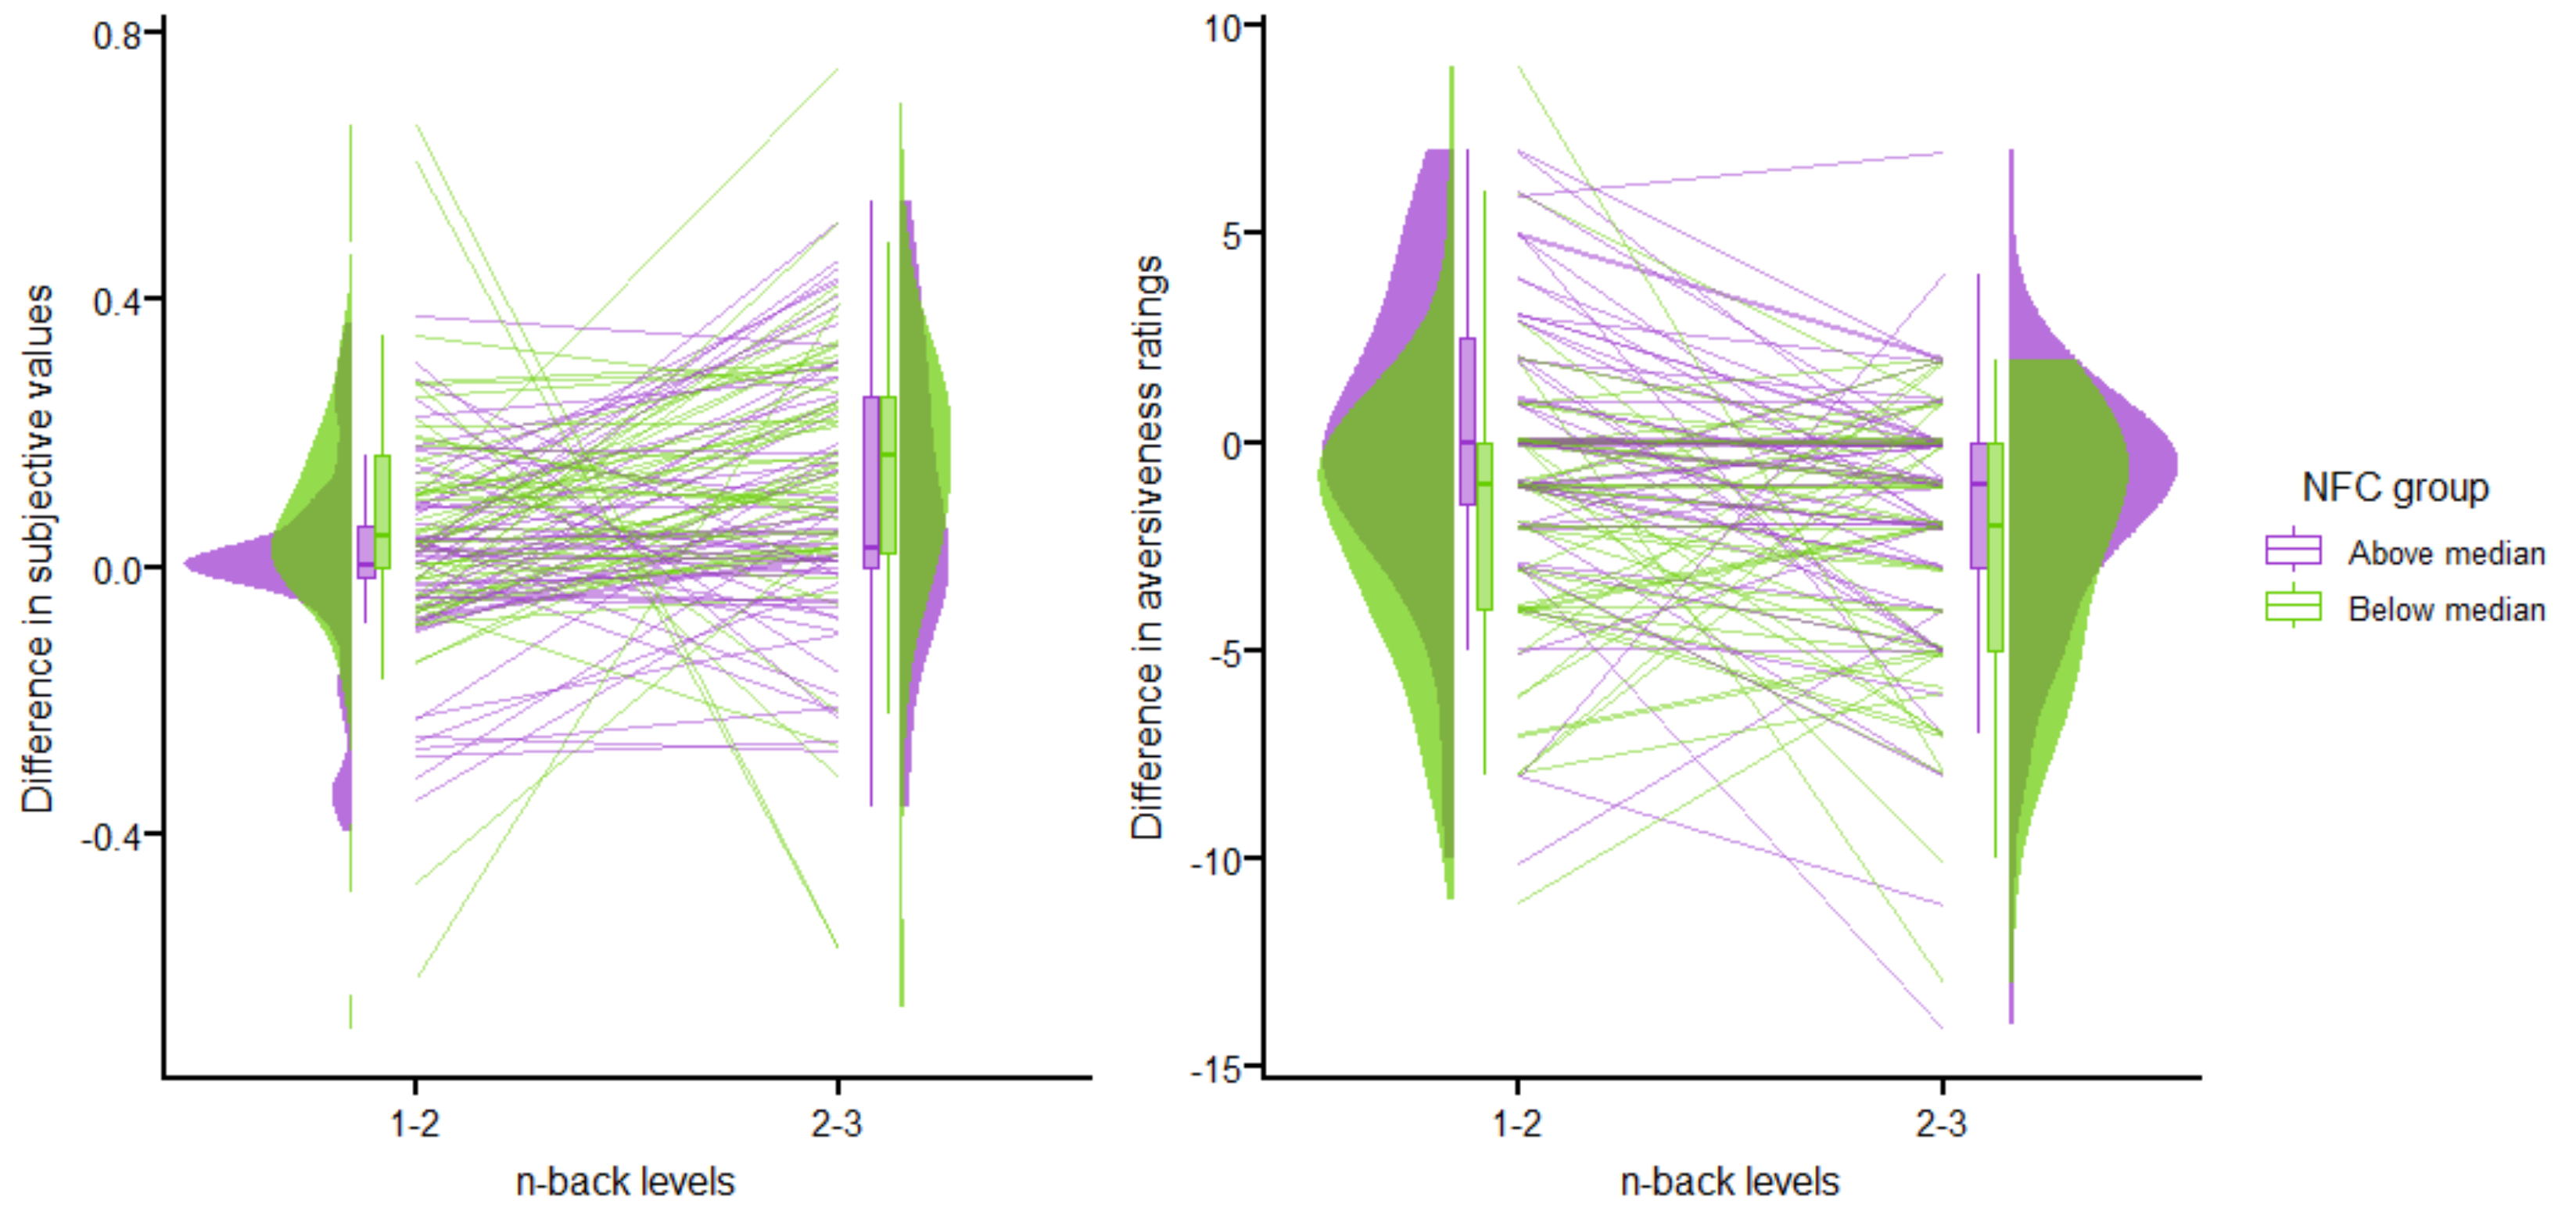
\includegraphics[width=\textwidth]{Figures/h3ac-plot} \caption{Difference scores for subjective values (a) and aversiveness ratings (b) when subtracting 2- from 1-back and 3- from 2-back. Horizontal lines of the boxplots represent the median per group, whiskers represent 1.5 interquartile ranges. NFC = Need for Cognition score. $N=116$. Figure available at osf.io/vnj8x/, under a CC-BY-4.0 license.}\label{fig:h3ac-plot}
\end{figure}

\newpage

\hypertarget{hypothesis-3b-participants-with-higher-nfc-scores-have-lower-nasa-tlx-scores-in-every-n-back-level-than-participants-with-lower-nfc-scores.}{%
\subsection{Hypothesis 3b: Participants with higher NFC scores have lower NASA-TLX scores in every n-back level than participants with lower NFC scores.}\label{hypothesis-3b-participants-with-higher-nfc-scores-have-lower-nasa-tlx-scores-in-every-n-back-level-than-participants-with-lower-nfc-scores.}}

ANOVA:

Main effect level: \(F(2.10, 239.56) = 154.50\), \(p < .001\), \(\hat{\eta}^2_G = .223\), 90\% CI \([.159, .282]\), \(\mathrm{BF}_{\textrm{10}} = 2.22 \times 10^{45}\)

Main effect NFC group: \(F(1, 114) = 3.22\), \(p = .075\), \(\hat{\eta}^2_G = .022\), 90\% CI \([.000, .084]\), \(\mathrm{BF}_{\textrm{10}} = 1.75 \times 10^{2}\)

Interaction: \(F(2.10, 239.56) = 4.93\), \(p = .007\), \(\hat{\eta}^2_G = .009\), 90\% CI \([.000, .025]\)

Contrast for main effect level:

\begin{table}[H]

\begin{center}
\begin{threeparttable}

\caption{\label{tab:unnamed-chunk-12}Paired contrasts for the rmANOVA comparing the influence of Need for Cognition group and $n$-back level on NASA-TLX scores.}

\begin{tabular}{lllllllll}
\toprule
Contrast & \multicolumn{1}{c}{Estimate} & \multicolumn{1}{c}{$SE$} & \multicolumn{1}{c}{$df$} & \multicolumn{1}{c}{$t$} & \multicolumn{1}{c}{$p$} & \multicolumn{1}{c}{$\mathrm{BF}_{\textrm{10}}$} & \multicolumn{1}{c}{$\eta_{p}^{2}$} & \multicolumn{1}{c}{$95\% CI$}\\
\midrule
1 - 2 & -1.86 & 0.18 & 114.00 & -10.06 & <.001 & $7.02 \times 10^{9}$ & 0.47 & {}[0.36, 1.00]\\
1 - 3 & -3.31 & 0.23 & 114.00 & -14.36 & <.001 & $6.43 \times 10^{29}$ & 0.64 & {}[0.56, 1.00]\\
1 - 4 & -3.82 & 0.25 & 114.00 & -15.32 & <.001 & $5.25 \times 10^{37}$ & 0.67 & {}[0.60, 1.00]\\
2 - 3 & -1.46 & 0.16 & 114.00 & -9.15 & <.001 & 113,671.29 & 0.42 & {}[0.31, 1.00]\\
2 - 4 & -1.96 & 0.19 & 114.00 & -10.39 & <.001 & $4.18 \times 10^{9}$ & 0.49 & {}[0.38, 1.00]\\
3 - 4 & -0.51 & 0.13 & 114.00 & -3.82 & 0.001 & 0.55 & 0.11 & {}[0.04, 1.00]\\
\bottomrule
\addlinespace
\end{tabular}

\begin{tablenotes}[para]
\normalsize{\textit{Note.} The column Contrast contains the $n$ of the $n$-back levels. $SE$ = standard error, $df$ = degrees of freedom, $t$ = $t$-statistic, $p$ = $p$-value, CI = confidence interval.}
\end{tablenotes}

\end{threeparttable}
\end{center}

\end{table}

Contrast for interaction:

\begin{table}[H]

\begin{center}
\begin{threeparttable}

\caption{\label{tab:unnamed-chunk-13}Paired contrasts for the rmANOVA comparing the influence of Need for Cognition group and $n$-back level on NASA-TLX scores.}

\begin{tabular}{llllllllll}
\toprule
Contrast & \multicolumn{1}{c}{Level} & \multicolumn{1}{c}{Estimate} & \multicolumn{1}{c}{$SE$} & \multicolumn{1}{c}{$df$} & \multicolumn{1}{c}{$t$} & \multicolumn{1}{c}{$p$} & \multicolumn{1}{c}{$\mathrm{BF}_{\textrm{10}}$} & \multicolumn{1}{c}{$\eta_{p}^{2}$} & \multicolumn{1}{c}{$95\% CI$}\\
\midrule
high - low & 1 & -0.23 & 0.48 & 114.00 & -0.48 & 0.632 & 0.18 & 2.02e-03 & {}[0.00, 1.00]\\
high - low & 2 & -0.40 & 0.53 & 114.00 & -0.76 & 0.450 & 0.25 & 5.00e-03 & {}[0.00, 1.00]\\
high - low & 3 & -1.14 & 0.53 & 114.00 & -2.15 & 0.033 & 11.15 & 0.04 & {}[0.00, 1.00]\\
high - low & 4 & -1.53 & 0.53 & 114.00 & -2.89 & 0.005 & 336.88 & 0.07 & {}[0.01, 1.00]\\
\bottomrule
\addlinespace
\end{tabular}

\begin{tablenotes}[para]
\normalsize{\textit{Note.} The column Contrast contains the groups above (high) and below (low) the Need for Cognition score median. $SE$ = standard error, $df$ = degrees of freedom, $t$ = $t$-statistic, $p$ = $p$-value, CI = confidence interval.}
\end{tablenotes}

\end{threeparttable}
\end{center}

\end{table}

\newpage

\begin{figure}[H]
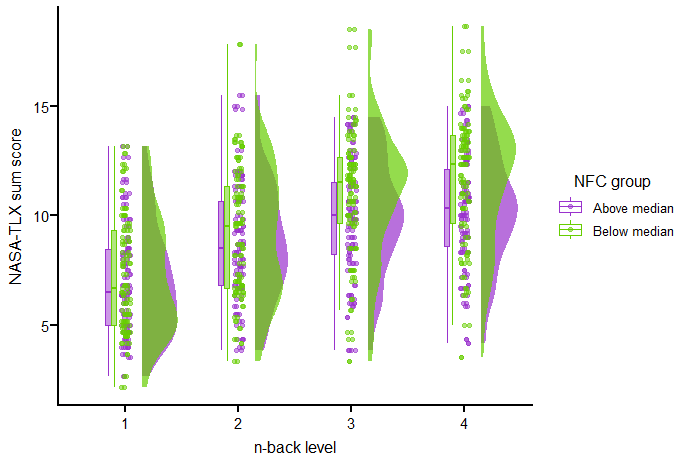
\includegraphics[width=\textwidth]{Figures/h3b-plot} \caption{NASA-TLX sum scores for each $n$-back level. Colours indicate Need for Cognition (NFC) score above or below the median. $N=116$. Figure available at osf.io/vnj8x/, under a CC-BY-4.0 license.}\label{fig:h3b-plot}
\end{figure}

\newpage

\hypertarget{hypothesis-3c-participants-with-higher-nfc-scores-have-lower-aversiveness-ratings-for-2--and-3-back-but-higher-higher-aversiveness-ratings-for-1-back-than-participants-with-lower-nfc-scores.}{%
\subsection{Hypothesis 3c: Participants with higher NFC scores have lower aversiveness ratings for 2- and 3-back but higher higher aversiveness ratings for 1-back than participants with lower NFC scores.}\label{hypothesis-3c-participants-with-higher-nfc-scores-have-lower-aversiveness-ratings-for-2--and-3-back-but-higher-higher-aversiveness-ratings-for-1-back-than-participants-with-lower-nfc-scores.}}

ANOVA:

Main effect level: \(F(1, 114) = 10.21\), \(p = .002\), \(\hat{\eta}^2_G = .034\), 90\% CI \([.000, .105]\),

Main effect NFC group: \(F(1, 114) = 8.43\), \(p = .004\), \(\hat{\eta}^2_G = .043\), 90\% CI \([.003, .119]\), \(\mathrm{BF}_{\textrm{10}} = 14.26\)

Interaction: \(F(1, 114) = 2.59\), \(p = .110\), \(\hat{\eta}^2_G = .009\), 90\% CI \([.000, .058]\)

Contrast for main effect level:

\begin{table}[H]

\begin{center}
\begin{threeparttable}

\caption{\label{tab:unnamed-chunk-14}Paired contrast for the rmANOVA comparing the influence of Need for Cognition group and $n$-back level on difference scores of aversiveness ratings.}

\begin{tabular}{lllllllll}
\toprule
Contrast & \multicolumn{1}{c}{Estimate} & \multicolumn{1}{c}{$SE$} & \multicolumn{1}{c}{$df$} & \multicolumn{1}{c}{$t$} & \multicolumn{1}{c}{$p$} & \multicolumn{1}{c}{$\mathrm{BF}_{\textrm{10}}$} & \multicolumn{1}{c}{$\eta_{p}^{2}$} & \multicolumn{1}{c}{$95\% CI$}\\
\midrule
1-2 - 2-3 & 1.27 & 0.40 & 114.00 & 3.20 & 0.002 & 5.49 & 0.08 & {}[0.02, 1.00]\\
\bottomrule
\addlinespace
\end{tabular}

\begin{tablenotes}[para]
\normalsize{\textit{Note.} The column Contrast contains the $n$ of the $n$-back levels. $SE$ = standard error, $df$ = degrees of freedom, $t$ = $t$-statistic, $p$ = $p$-value, CI = confidence interval.}
\end{tablenotes}

\end{threeparttable}
\end{center}

\end{table}

Contrast for main effect NFC group:

\begin{table}[H]

\begin{center}
\begin{threeparttable}

\caption{\label{tab:unnamed-chunk-15}Paired contrast for the rmANOVA comparing the influence of Need for Cognition (NFC) group and $n$-back level on difference scores of aversiveness ratings.}

\begin{tabular}{lllllllll}
\toprule
Contrast & \multicolumn{1}{c}{Estimate} & \multicolumn{1}{c}{$SE$} & \multicolumn{1}{c}{$df$} & \multicolumn{1}{c}{$t$} & \multicolumn{1}{c}{$p$} & \multicolumn{1}{c}{$\mathrm{BF}_{\textrm{10}}$} & \multicolumn{1}{c}{$\eta_{p}^{2}$} & \multicolumn{1}{c}{$95\% CI$}\\
\midrule
High NFC - Low NFC & 1.44 & 0.50 & 114.00 & 2.90 & 0.004 & 14.26 & 0.07 & {}[0.01, 1.00]\\
\bottomrule
\addlinespace
\end{tabular}

\begin{tablenotes}[para]
\normalsize{\textit{Note.} $SE$ = standard error, $df$ = degrees of freedom, $t$ = $t$-statistic, $p$ = $p$-value, CI = confidence interval.}
\end{tablenotes}

\end{threeparttable}
\end{center}

\end{table}

\newpage

\hypertarget{exploratory-analysis-with-nfc-groups-by-median-split}{%
\subsection{Exploratory analysis with NFC groups by median split}\label{exploratory-analysis-with-nfc-groups-by-median-split}}

ANOVA:

Main effect level: \(F(2.01, 229.39) = 67.39\), \(p < .001\), \(\hat{\eta}^2_G = .295\), 90\% CI \([.228, .354]\), \(2.70 \times 10^{30}\)

Main effect NFC group: \(F(1, 114) = 2.63\), \(p = .108\), \(\hat{\eta}^2_G = .007\), 90\% CI \([.000, .053]\), \(2.95 \times 10^{-1}\)

Interaction: \(F(2.01, 229.39) = 3.24\), \(p = .041\), \(\hat{\eta}^2_G = .020\), 90\% CI \([.000, .044]\)

Contrasts for main effect level:

\begin{table}[H]

\begin{center}
\begin{threeparttable}

\caption{\label{tab:unnamed-chunk-16}Paired contrast for the rmANOVA comparing the influence of Need for Cognition group and $n$-back level on subjective values.}

\begin{tabular}{lllllllll}
\toprule
Contrast & \multicolumn{1}{c}{Estimate} & \multicolumn{1}{c}{$SE$} & \multicolumn{1}{c}{$df$} & \multicolumn{1}{c}{$t$} & \multicolumn{1}{c}{$p$} & \multicolumn{1}{c}{$\mathrm{BF}_{\textrm{10}}$} & \multicolumn{1}{c}{$\eta_{p}^{2}$} & \multicolumn{1}{c}{$95\% CI$}\\
\midrule
1 - 2 & 0.03 & 0.02 & 114.00 & 2.03 & 0.184 & 0.66 & 0.03 & {}[0.00, 1.00]\\
1 - 3 & 0.15 & 0.03 & 114.00 & 5.77 & <.001 & 117,986.95 & 0.23 & {}[0.12, 1.00]\\
1 - 4 & 0.33 & 0.03 & 114.00 & 9.70 & <.001 & $1.47 \times 10^{13}$ & 0.45 & {}[0.34, 1.00]\\
2 - 3 & 0.11 & 0.02 & 114.00 & 5.55 & <.001 & 67,167.07 & 0.21 & {}[0.11, 1.00]\\
2 - 4 & 0.30 & 0.03 & 114.00 & 10.22 & <.001 & $4.31 \times 10^{14}$ & 0.48 & {}[0.37, 1.00]\\
3 - 4 & 0.19 & 0.03 & 114.00 & 7.30 & <.001 & $1.68 \times 10^{8}$ & 0.32 & {}[0.21, 1.00]\\
\bottomrule
\addlinespace
\end{tabular}

\begin{tablenotes}[para]
\normalsize{\textit{Note.} The column Contrast contains the $n$ of the $n$-back levels. $SE$ = standard error, $df$ = degrees of freedom, $t$ = $t$-statistic, $p$ = $p$-value, CI = confidence interval.}
\end{tablenotes}

\end{threeparttable}
\end{center}

\end{table}

Contrasts for the interaction:

\begin{table}[H]

\begin{center}
\begin{threeparttable}

\caption{\label{tab:unnamed-chunk-17}Paired contrast for the rmANOVA comparing the influence of Need for Cognition group and $n$-back level on subjective values.}

\begin{tabular}{llllllllll}
\toprule
Contrast & \multicolumn{1}{c}{Level} & \multicolumn{1}{c}{Estimate} & \multicolumn{1}{c}{$SE$} & \multicolumn{1}{c}{$df$} & \multicolumn{1}{c}{$t$} & \multicolumn{1}{c}{$p$} & \multicolumn{1}{c}{$\mathrm{BF}_{\textrm{10}}$} & \multicolumn{1}{c}{$\eta_{p}^{2}$} & \multicolumn{1}{c}{$95\% CI$}\\
\midrule
high - low & 1 & -0.05 & 0.03 & 114.00 & -1.50 & 0.136 & 0.54 & 0.02 & {}[0.00, 1.00]\\
high - low & 2 & 0.02 & 0.03 & 114.00 & 0.72 & 0.472 & 0.25 & 4.54e-03 & {}[0.00, 1.00]\\
high - low & 3 & 0.05 & 0.04 & 114.00 & 1.28 & 0.203 & 0.41 & 0.01 & {}[0.00, 1.00]\\
high - low & 4 & 0.11 & 0.05 & 114.00 & 2.13 & 0.036 & 1.48 & 0.04 & {}[0.00, 1.00]\\
\bottomrule
\addlinespace
\end{tabular}

\begin{tablenotes}[para]
\normalsize{\textit{Note.} The column Contrast contains the groups above (high) and below (low) the Need for Cognition score median. The column Level contains the $n$ of the $n$-back levels. $SE$ = standard error, $df$ = degrees of freedom, $t$ = $t$-statistic, $p$ = $p$-value, CI = confidence interval.}
\end{tablenotes}

\end{threeparttable}
\end{center}

\end{table}

\newpage

\hypertarget{exploratory-analysis-with-nfc-as-a-continuous-covariate}{%
\subsection{Exploratory analysis with NFC as a continuous covariate}\label{exploratory-analysis-with-nfc-as-a-continuous-covariate}}

ANOVA (NFC scores standardized):

\begin{table}[H]

\begin{center}
\begin{threeparttable}

\caption{\label{tab:unnamed-chunk-18}Result of the rmANOVA regarding the predictive power of the $n$-back level on the subjective values when including Need for Cognition scores as a centered continuous covariate.}

\begin{tabular}{lllllllll}
\toprule
 & \multicolumn{1}{c}{Sum Sq} & \multicolumn{1}{c}{$df$} & \multicolumn{1}{c}{error Sum Sq} & \multicolumn{1}{c}{den $df$} & \multicolumn{1}{c}{$F$} & \multicolumn{1}{c}{$p$} & \multicolumn{1}{c}{$\eta_{p}^{2}$} & \multicolumn{1}{c}{$95\% CI$}\\
\midrule
Intercept & 301.49 & 1.00 & 5.44 & 114.00 & 6,322.13 & <.001 & 0.98 & {}[0.98, 1.00]\\
NFC & 0.21 & 1.00 & 5.44 & 114.00 & 4.34 & 0.039 & 0.04 & {}[0.00, 1.00]\\
n-back level & 7.83 & 3.00 & 13.28 & 342.00 & 67.24 & <.001 & 0.37 & {}[0.30, 1.00]\\
NFC x n-back level & 0.44 & 3.00 & 13.28 & 342.00 & 3.78 & 0.011 & 0.03 & {}[0.00, 1.00]\\
\bottomrule
\addlinespace
\end{tabular}

\begin{tablenotes}[para]
\normalsize{\textit{Note.} NFC = Need for Cognition. $SE$ = standard error, $df$ = degrees of freedom, $F$ = $F$-statistic, $p$ = $p$-value, $\eta_{p}^{2}$ = partial eta squared, CI = confidence interval.}
\end{tablenotes}

\end{threeparttable}
\end{center}

\end{table}

Estimated marginal means of the linear trends:

\begin{table}[H]

\begin{center}
\begin{threeparttable}

\caption{\label{tab:unnamed-chunk-19}Paired contrast slope analysis as a follow up for the rmANOVA regarding the predictive power of the $n$-back level on the subjective values when including Need for Cognition scores as a centered continuous covariate.}

\begin{tabular}{llllll}
\toprule
$n$-back level & \multicolumn{1}{c}{Estimate} & \multicolumn{1}{c}{$SE$} & \multicolumn{1}{c}{$df$} & \multicolumn{1}{c}{$t$} & \multicolumn{1}{c}{$p$}\\
\midrule
1 - 2 & -0.03 & 0.03 & 456.00 & -1.11 & 0.68\\
1 - 3 & -0.03 & 0.03 & 456.00 & -1.27 & 0.58\\
1 - 4 & -0.09 & 0.03 & 456.00 & -3.22 & 0.01\\
2 - 3 & 0.00 & 0.03 & 456.00 & -0.16 & 1.00\\
2 - 4 & -0.06 & 0.03 & 456.00 & -2.10 & 0.15\\
3 - 4 & -0.05 & 0.03 & 456.00 & -1.95 & 0.21\\
\bottomrule
\addlinespace
\end{tabular}

\begin{tablenotes}[para]
\normalsize{\textit{Note.} The column $n$-back level contains the $n$ of the task levels. $SE$ = standard error, $df$ = degrees of freedom, $t$ = $t$-statistic, $p$ = $p$-value.}
\end{tablenotes}

\end{threeparttable}
\end{center}

\end{table}

\newpage

\begin{figure}[H]
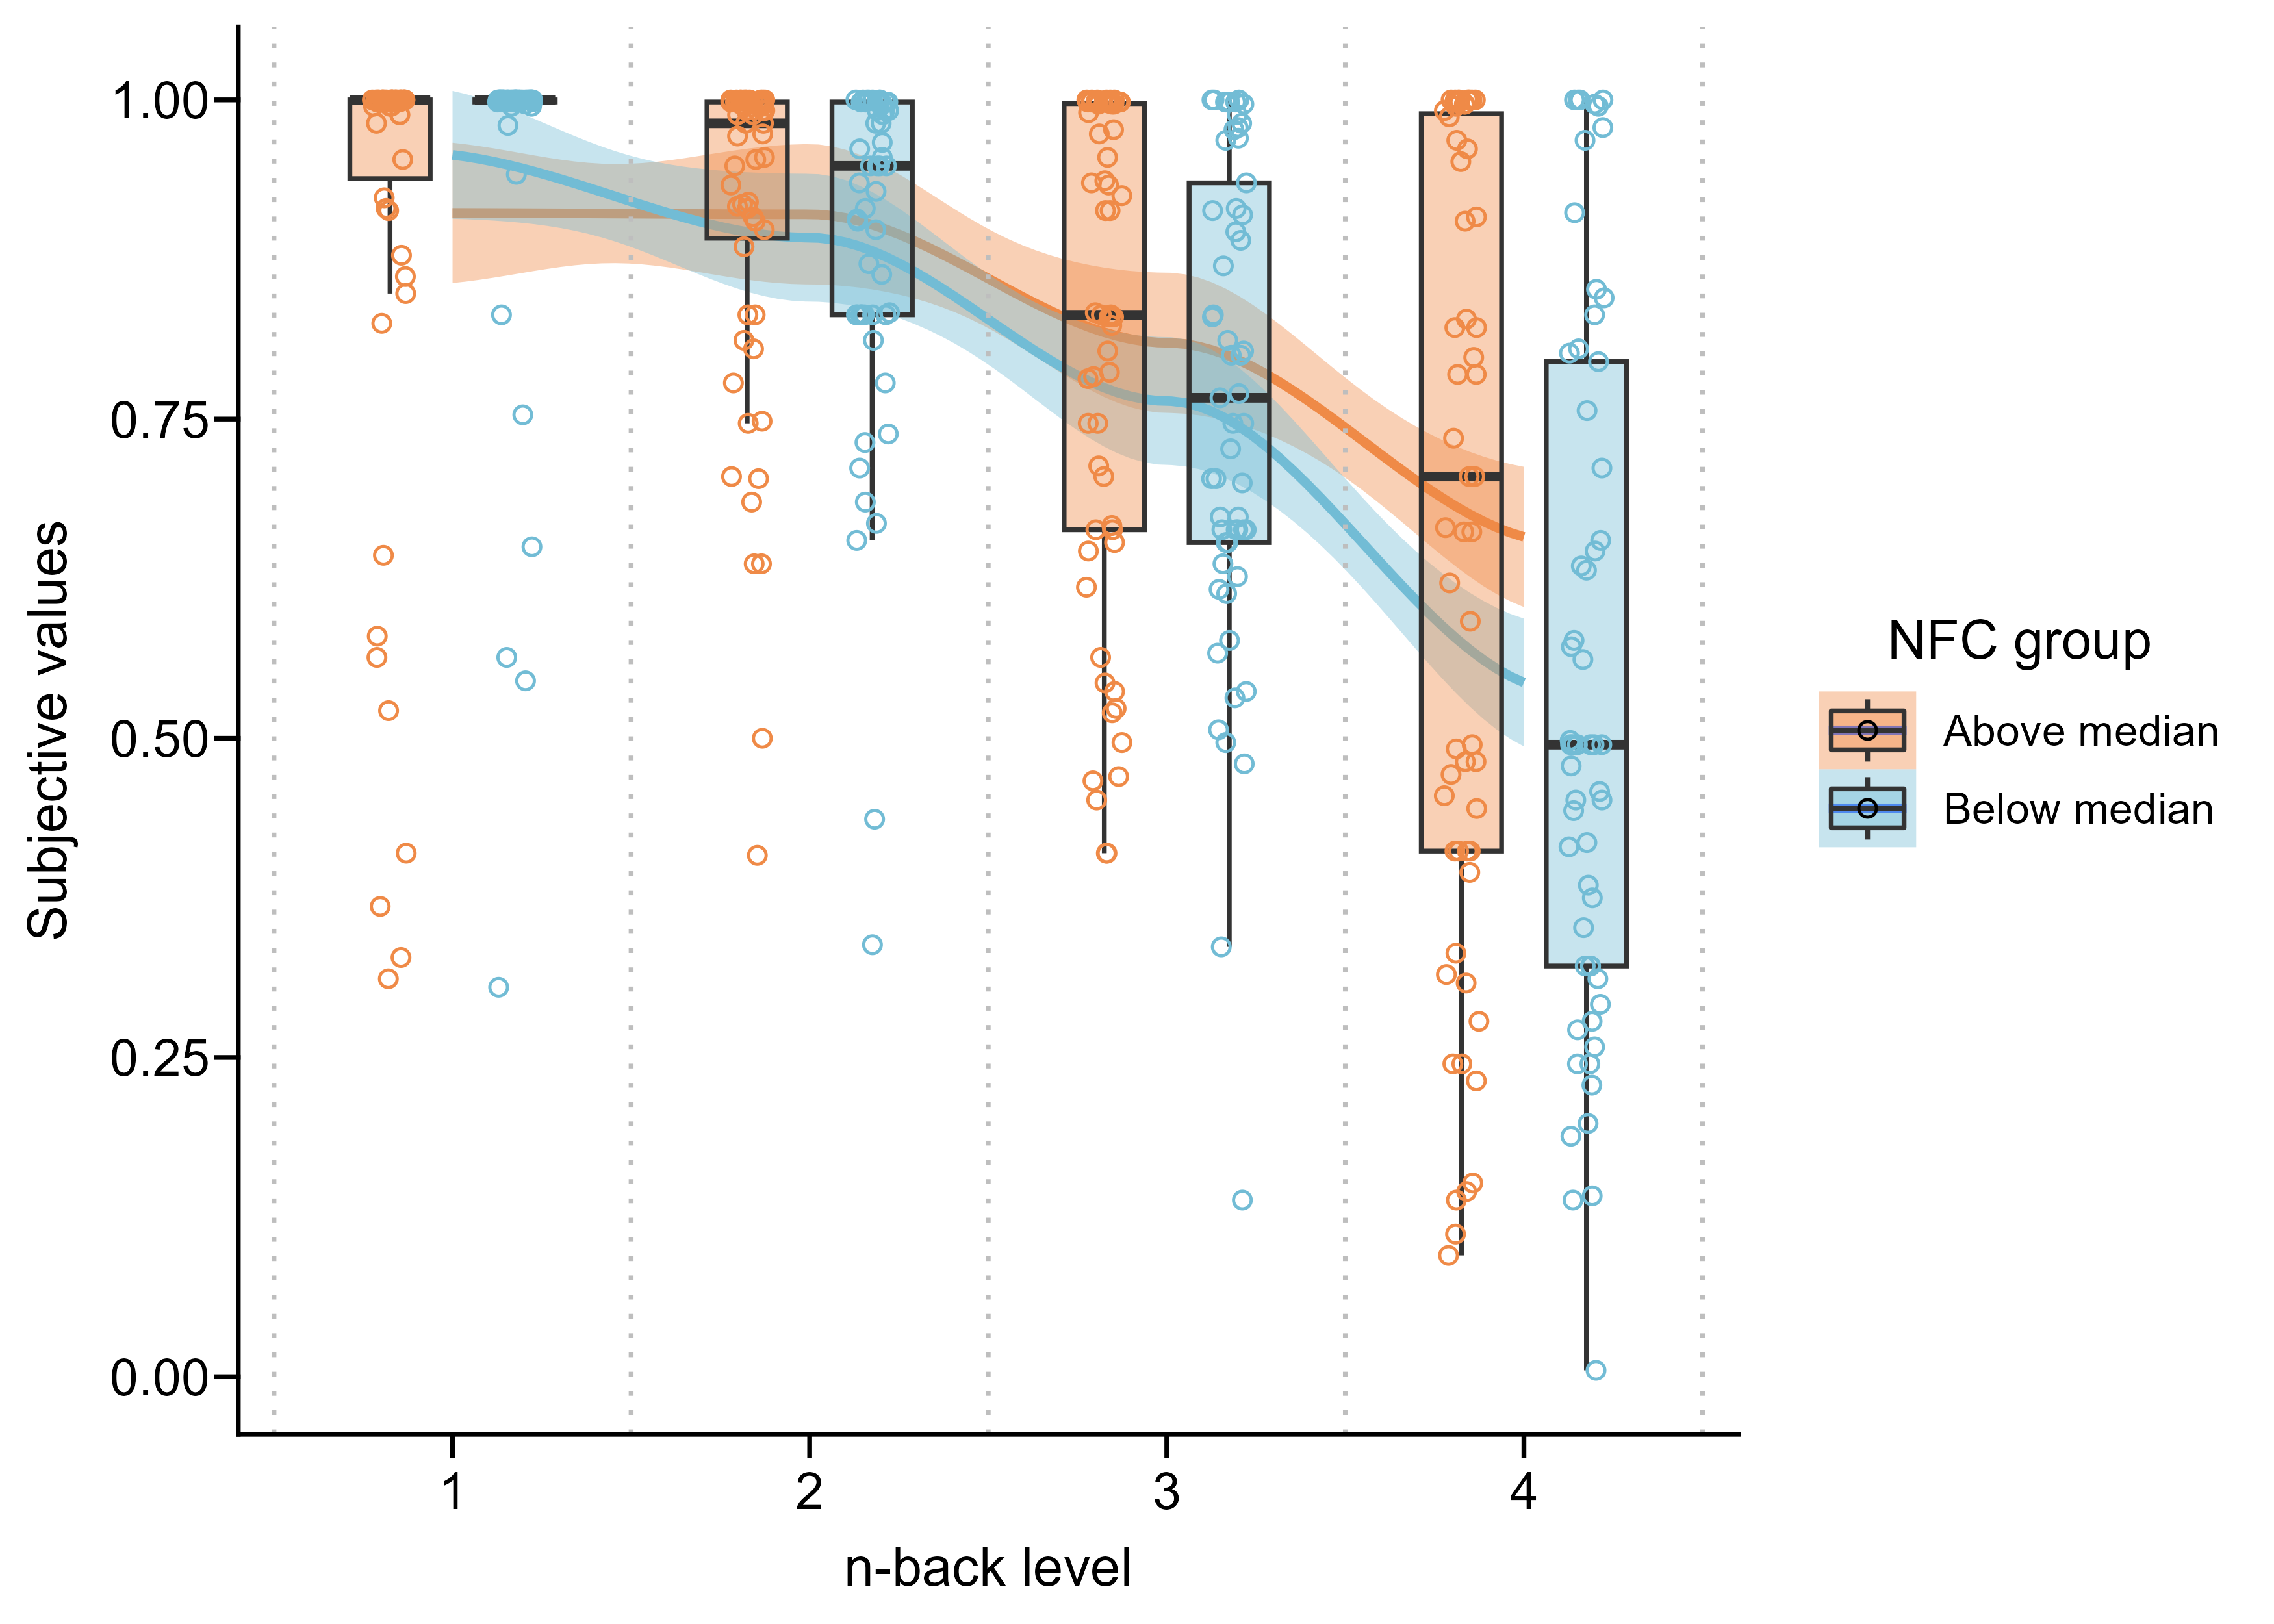
\includegraphics[width=\textwidth]{Figures/nfcgroups-sv} \caption{Subjective values per n-back level for participants with Need for Cognition (NFC) scores above and below the median. $N=116$. The scatter has a horizontal jitter of 0.2. Smoothing of conditional means with Loess method. Figure available at osf.io/vnj8x/, under a CC-BY-4.0 license.}\label{fig:nfcgroups-sv}
\end{figure}


\end{document}
